\addsec{Vorlesung 12 - Leitungscodes, WLAN}

\minisec{Erklären Sie den Begriff Signalbildung (bzw. Leitungskodierung)!}
\begin{itemize}
    \item \todo A
\end{itemize}

\minisec{Welche Anforderungen kennen Sie, die ein guter Leitungscode erfüllen sollte?}
\begin{itemize}
    \item Möglichst hohe \textcolor{blue}{Widerstandsfähigkeit gegen Dämpfung}
    \item \textcolor{blue}{Effizienz:} möglichst hohe Übertragungsraten durch Codewörter
    \begin{itemize}
        \item binärer Code: +5V / -5V?
        \item ternärer Code: +5 V / 0V / -5V?
        \item quaternärer Code: 4 Zustände (Codierung von 2 Bit gleichzeitig)
    \end{itemize}
    \item \textcolor{blue}{Taktrückgewinnung} beim Empfänger (\textcolor{blue}{Synchronisation}), dazu möglichst
    häufige/regelmäßige Pegelwechsel
    \item Gleichstromfreiheit: positive und negative Signale treten ungefähr gleich oft auf → kein nennenswerter elektrischer Gleichstrom-Fluss
    \item Robustheit: Können längere Sequenzen von 0 und 1 noch als solche noch erkannt werden?
    Können fehlerhafte Bits erkannt werden?
\end{itemize}

\minisec{Welche Vor- und Nachteile hat ein binärer gegenüber einem quaternären Code?}
\begin{itemize}
    \item \todo A
\end{itemize}

\minisec{Erklären Sie den Unterschied zwischen Basisband- und Breitband-Übertragung!}
\begin{itemize}
    \item \textcolor{blue}{Basisband:} Das Basisband ist der natürliche Frequenzbereich des Nutzsignals (untere Grenzfrequenz $f_{min}$ gleich oder nahe bei 0 Hz).
    Die digitalen Informationen werden ‚direkt‘ in physikalische Größen übersetzt und so über die Leitung übertragen.
    Hierzu sind Kodierungsverfahren notwendig, die festlegen, wie bei der Übertragung eine 0 bzw.\ eine 1 repräsentiert werden.
    Es kann nur je ein Signal übertragen werden
    \item \textcolor{blue}{Breitband:} Die digitalen Nutzdaten werden nicht direkt übertragen, sondern einem oder mehreren hochfrequenten Trägern aufmoduliert.
    Durch die Verwendung verschiedener Trägerwellen (Frequenzen) können dann mehrere Informationen gleichzeitig übermittelt werden
\end{itemize}

\minisec{Erklären Sie den Unterschied zwischen Bit- und Baudrate!}
\begin{itemize}
    \item Wenn die Zeitdauer (Schrittdauer) eines \textcolor{blue}{Symbols} bzw.\ \textcolor{blue}{Codeelements} $T$ ist,
    ist die Schrittgeschwindigkeit \[v_s = \frac{1}{T}\] (Einheit: \textcolor{blue}{Baud}), Symbolrate
    \item Die Übertragungsgeschwindigkeit (äquivalente Bitrate) ist dann \[v_u = v_s ld n\] ($n=$ Anzahl diskreter Zustände des Codeelements)
\end{itemize}
Bei binären Codeelementen stimmen somit \textcolor{blue}{Bitrate} und \textcolor{blue}{Baudrate} (Schrittgeschwindigkeit) überein, falls nur Codeelemente für Daten übermittelt werden (es gibt auch Codeelemente für z.\ B. die Rahmenstruktur)

\minisec{Was ist der Unterschied zwischen einem NRZ- und einem RZ-Code?}
\begin{itemize}
    \item \textbf{NRZ / NRZ-L: Non-Return\_to\_Zero:}
    \begin{itemize}
        \item Kein automatisches Zurückfallen auf einen Grundpegel.
        Hier z.\ B.:
        \item 0 = negative Spannung (konstant 0V), Pegel 1
        \item 1 = positive Spannung (konstant +5V), Pegel 2
        \item \underline{Nachteil:} bei langen 0 oder 1 Folgen \underline{Taktverlust} und \underline{keine Gleichstromfreiheit}
        \item \underline{Beispiel:} UART, RS232 (serielle Schnittstellen)
    \end{itemize}
    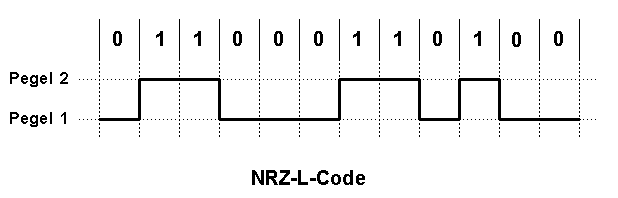
\includegraphics[width=0.8\textwidth]{img/NRZ-L-Code}
    \item \textbf{RZ: Return to Zero (hier unipolar)}
    \begin{itemize}
        \item 0 = 0V
        \item 1 = $\frac{T}{2}$ lang 1, $\frac{T}{2}$ lang 0
        \item \underline{Vorteil:} Taktrückgewinnung bei 1-Folgen
        \item \underline{Nachteil:} Keine Gleichstromfreiheit, kein Takt bei langen 0-Folgen
        \item \underline{Beispiel:} IrDA – Fernbedienung
    \end{itemize}
    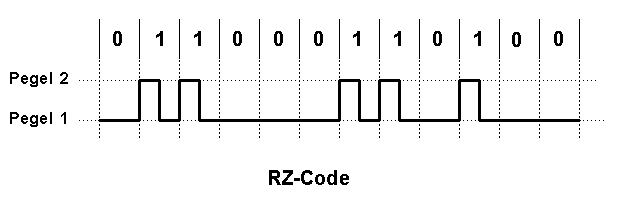
\includegraphics[width=0.8\textwidth]{img/RZ-Code}
\end{itemize}

\minisec{Welche Eigenschaften besitzt der Manchester-Code? Was bedeutet 1B2B?
Wie unterscheiden sich die Standards nach G.E. Thomas und IEEE 802.3?}
\begin{itemize}
    \item Eigenschaften:
    \begin{itemize}
        \item Lange Folgen gleicher Signale werden durch einen Pegelwechsel in
        der Mitte jedes Bits verhindert.
        Nach G.\ E. Thomas:
        \item 0 = Polaritätswechsel von negativ (-5V) nach positiv (+5V)
        \item 1 = Polaritätswechsel von positiv (+5V) nach negativ (-5V)
        \item \underline{Vorteil:} Gleichstromfrei, Taktrückgewinnung möglich
        \item \underline{Nachteil:} Doppelte Bandbreite im Vergleich zu NRZ, Bitrate $= \frac{Baudrate}{2}$
        \item \underline{Beispiel:} 10Base2
    \end{itemize}
    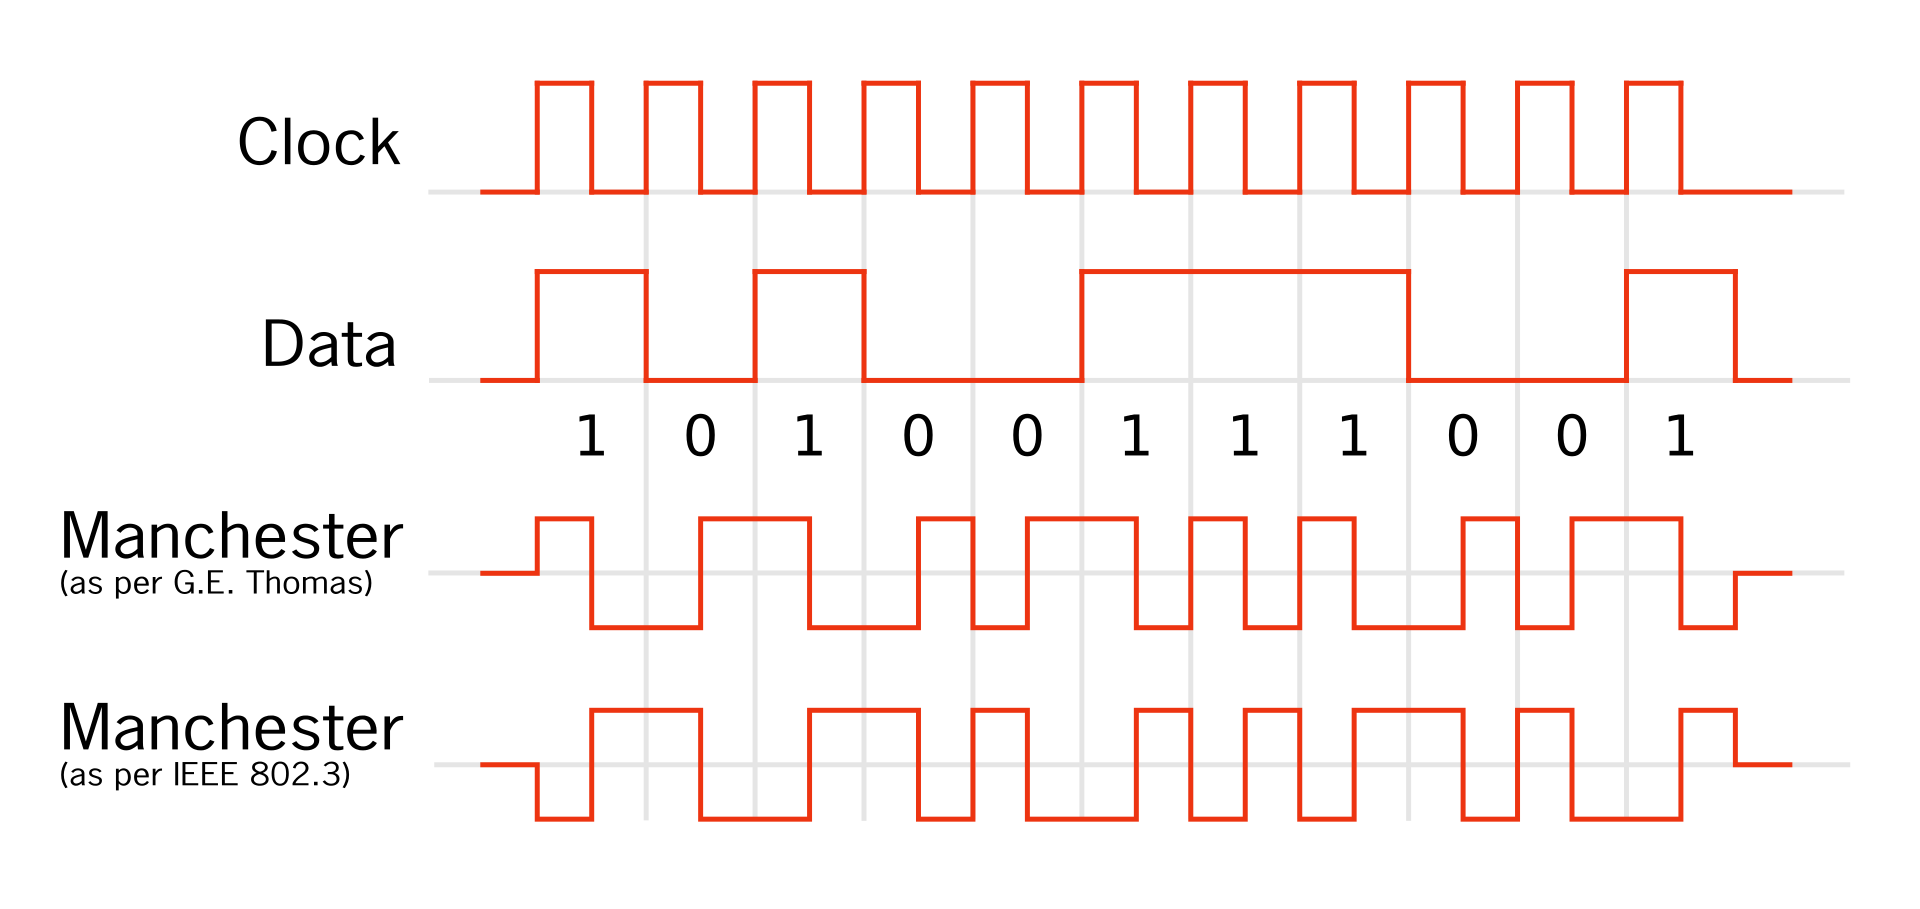
\includegraphics[width=\textwidth]{img/Manchester-Code}
    \item \textcolor{blue}{1B/2B-:} ein Bit wird auf zwei Symbole kodiert
\end{itemize}

\minisec{Welche Vorteile hat ein 4B/5B Code gegenüber einem 1B/2B Code?}
\begin{itemize}
    \item \underline{Nachteil des Manchester-Codes:}
    \begin{itemize}
        \item 50\% Effizienz, d.\ h. \textcolor{blue}{1B/2B-Code} (ein Bit wird auf zwei Symbole kodiert)
        Eine Verbesserung stellt der \textcolor{blue}{4B/5B-Code} dar:
        \item vier Bit werden in fünf Symbole kodiert: 80\% Effizienz
    \end{itemize}
    \item \underline{Arbeitsweise:}
    \begin{itemize}
        \item Pegelwechsel bei 1, kein Pegelwechsel bei 0 (Differentieller NRZ-Code)
        \item Kodierung von hexadezimalen Zeichen: 0, 1,\ldots, 9, A, B,\ldots, F (4 Bit)
        in 5 Bit, sodass lange Nullenblöcke vermieden werden.
        \item Auswahl der günstigsten 16 der möglichen 32 Codewörter
        (maximal 3 Nullen in Folge)
        \item Weitere 5 Bit-Kombinationen für Steuerinformationen
        \item Erweiterbar auf 1000B/1001B-Codes?
    \end{itemize}
\end{itemize}

\minisec{Welche Eigenschaften eines Trägersignals können zur Modulation verwendet werden?}
\begin{itemize}
    \item Amplitude
    \item Frequenz
    \item Signale
    \item $s(t) = A \cdot \sin(2 \cdot \pi \cdot f \cdot t + \phi)$
\end{itemize}

\minisec{Welche Möglichkeiten kennen Sie, um bei einer Breitbandübertragung die Datenrate zu erhöhen?}
\begin{itemize}
    \item \todo A
\end{itemize}

\minisec{Warum ist PSK weniger störanfällig als z.B. ASK?}
\begin{itemize}
    \item \todo A
\end{itemize}

\minisec{Wie unterscheiden sich QPSK und QAM?}
\begin{itemize}
    \item \textcolor{blue}{BPSK} (Binary Phase Shift Keying):
    \begin{itemize}
        \item $=$ einfaches PSK
        \item $>$ Bitwert 0: Sinuswelle
        \item $>$ Bitwert 1: invertierte Sinuswelle
        \item Niedrige Datenraten
        \item Robuste Übertragung
        \item Auch oft als differentieller Code (DBPSK)
    \end{itemize}
    \item \textcolor{blue}{QPSK} (Quaternary Phase Shift Keying):
    \begin{itemize}
        \item Zwei Bit werden gemeinsam codiert
        \item Vier unterschiedliche Phasenlagen
        \item Doppelte Datenraten verglichen mit BPSK
    \end{itemize}
\end{itemize}

\minisec{Welche Störeinflüsse gibt es bei der Datenübertragung mit Funkwellen?}
\begin{itemize}
    \item natürliche Umgebung: Gebirge, Wasser, Vegetation, Regen, Schnee
    \item künstliche Umgebung: Gebäude etc.
\end{itemize}

\minisec{Worin unterscheidet sich ein kabelgebundenes gemeinsames Medium (z.B. ein Bus bei 10Base2) von einem funkbasierten 'gemeinsamen' Medium (Luftraum bei WLAN)?}
\begin{itemize}
    \item \todo A
\end{itemize}

\minisec{Wie groß sind typische Übertragungsraten beim WLAN?
Welche Frequenzbänder werden benutzt?}
\begin{itemize}
    \item Datenraten:
    \begin{itemize}
        \item 1, 2, 5.5, 11, 6, 9, 12, 18, 24, 36, 48, 54, \ldots MBit/s Bruttodatenrate
        \item Abhängig von Signalqualität wird die bestmögliche Datenrate gewählt
        \item Nutzdatenrate wenig mehr als die Hälfte der jeweiligen Bruttodatenrate
    \end{itemize}
    \item Frequenzbereich:
    \begin{itemize}
        \item Freies 2.4 GHz-Band (2.4 - 2.4835 GHz) ISM = Industrial – Scientific – Medical
        \item Optional 5 GHz-Band
    \end{itemize}
\end{itemize}

\minisec{Warum ist das CSMA/CD-Verfahren bei WLAN nur schwer anwendbar?}
Zentral hierbei ist das Hidden-Station-Problem.
Dies tritt auf, wenn zwei Stationen sich gegenseitig nicht wahrnehmen, aber gleichzeitig mit einer dritten Station in der Mitte kommunizieren – was unweigerlich zu Kollisionen führt.

\minisec{Erklären Sie das 'Hidden Station'-Problem bei WLAN!}
\begin{itemize}
    \item A sendet an B, C empfängt A nicht
    \item C will an B senden, stellt freies Medium fest (CS schlägt fehl)
    \item Kollision bei B, A bemerkt sie nicht (CD schlägt fehl)
    \item A ist \textcolor{blue}{hidden} (versteckt) für C
\end{itemize}

\minisec{Erklären Sie das 'Exposed-Station'-Problem bei WLAN!}
\begin{itemize}
    \item B sendet zu A, C will zu D senden
    \item C muss warten, da CS ein „besetztes“ Medium signalisiert
    \item da A aber außerhalb der Reichweite von C ist, ist dies unnötig A
\end{itemize}

\minisec{Erklären Sie grob das Vorgehen bei CSMA/CA! Wie werden Kollisionen verhindert?}
\begin{itemize}
    \item \textcolor{blue}{Carrier Sense Multiple Access with Collision Avoidance}
    \item Kollisionen können nicht erkannt werden, darum wird versucht, sie zu vermeiden
    \item Carrier Sense mit zufallsgetriebenen Backoff-Mechanismus
    \item Kollisionsvermeidung Idee:
    \begin{itemize}
        \item Vor Beginn des Sendens: \textcolor{blue}{Carrier Sense}
        \item Falls Medium frei für mindestens eine Zeit von DIFS, starte direkt mit Übertragung
        \item Falls Medium belegt: warte bei Freiwerden erneut für DIFS, wähle dann eine Backoff-Zeit vor nächsten Zugriffsversuch (\textcolor{blue}{Kollisionsvermeidung})
        \begin{itemize}
            \item Backoff-Zeit ist Vielfaches eines Zeitslots
        \end{itemize}
    \end{itemize}
    \item Kollisionsvermeidung Vorgehen:
    \begin{itemize}
        \item Falls Medium nach Ablauf der Backoff-Zeit noch immer frei,
        starte mit Übertragung
        \item Falls Medium eher belegt wird:
        \begin{itemize}
            \item Stoppe Backoff-Zähler
            \item Verwende aktuellen Wert beim nächsten Versuch weiter
        \end{itemize}
    \end{itemize}
    \item Quittierung jeder Übertragung, da Kollisionen nicht erkannt werden können
    \begin{itemize}
        \item \textcolor{blue}{Direkte} Bestätigung jedes korrekten Datenrahmens
        \begin{itemize}
            \item Wichtige Kontrollinformation, daher werden diese bereits nach SIFS ohne jegliches Backoff versendet
        \end{itemize}
    \end{itemize}
\end{itemize}